\documentclass[hyperref, UTF8]{ctexart}
\usepackage{graphicx}
\usepackage{float}
\usepackage{amsmath}
\usepackage{amsfonts}
\usepackage{amssymb}
\usepackage{fontspec}
\usepackage{tikz}
\setmonofont{Monaco}
\setCJKmainfont{PingFang SC Regular}
\usetikzlibrary{shapes.geometric, arrows}
\tikzstyle{startstop} = [rectangle, rounded corners, minimum width=3cm, minimum height=1cm,text centered, draw=black, fill=red!30]
\tikzstyle{io} = [trapezium, trapezium left angle=70, trapezium right angle=110, minimum width=3cm, minimum height=1cm, text centered, draw=black, fill=blue!30]
\tikzstyle{process} = [rectangle, minimum width=3cm, minimum height=1cm, text centered, draw=black, fill=orange!30]
\tikzstyle{decision} = [diamond, minimum width=3cm, minimum height=1cm, text centered, draw=black, fill=green!30]
\tikzstyle{arrow} = [thick,->,>=stealth]
\usepackage[a4paper, top=3cm, bottom=3cm, left=3cm, right=3cm]{geometry}
\usepackage{subcaption}
\usepackage{xcolor}
\usepackage{listings}
\lstset{
	keywordstyle=\color{blue!70},
	commentstyle=\color{red!50!green!50!blue!50},
	frame=shadowbox,
	rulesepcolor=\color{red!20!green!20!blue!20},
	tabsize=2,
	basicstyle=\ttfamily\small,
	numberstyle=\tiny,
	numbers=left,
	showstringspaces=false,
	breaklines=true,
	language=MATLAB
}
\hypersetup{
	colorlinks=true,
	bookmarks=true,
	bookmarksopen=true,
	pdftitle=遥感综合实验~遥感信号处理处理实验报告,
	pdfauthor=16020710017~蓝彧文,
	linkcolor=blue
}
\newcommand{\rect}{\mathrm{rect}}
\newcommand{\rectf}[1]{\mathrm{rect}\left( #1 \right)}
\newcommand{\sinc}{\mathrm{sinc}}
\newcommand{\jj}{\mathrm{j}}
\newcommand{\abs}[1]{\left| #1 \right|}
\newcommand{\dd}{\mathrm{dd}}
\newcommand{\singleimage}[2]{\begin{figure}[H]\centering\includegraphics[width=0.7\linewidth]{#1}\caption{#2} \end{figure}}
\newcommand{\doubleimages}[4]{\begin{figure}[H]
		\centering
		\begin{minipage}{0.45\linewidth}
			\centering
			\includegraphics[width=\linewidth]{#1}
			\caption{#2} 
		\end{minipage}
		\begin{minipage}{0.45\linewidth}
			\centering
			\includegraphics[width=\linewidth]{#3}
			\caption{#4} 
		\end{minipage}
\end{figure}}
\title{遥感综合实验实验报告\\遥感信号处理}
\author{蓝彧文~16020710017}
\begin{document}
	\maketitle
	\tableofcontents
	\newpage
	实验中使用的所有代码和数据可以在\\ \url{https://github.com/EwenLan/remote-sensing-library}获取。
	\section{实验十一~线性调频信号的脉冲压缩}
	\subsection{实验目的}
理解遥感信号处理的概念,学习雷达信号处理中的线性调频信号及其脉冲压缩技术。通过实验了解线性调频信号的性质,并实现线性调频信号的脉冲压缩。
\subsection{实验原理}
\subsubsection{离散时间信号的线性卷积}

\begin{equation}
\begin{split}
y(n) =& s(n) \otimes h(n) \\
=& \sum_{m=0}^{M-1} s(n - m)h(m) \\
=& \sum_{m=n-(M-1)}^{n} s(m)h(n - m) \\
\end{split}
\end{equation}
\subsubsection{傅立叶变换的性质}
\begin{eqnarray}
g_1(t)\otimes g_2(t) &\leftrightarrow& G_1(f)G_2(f) \\
g_1(t)g_2(t) &\leftrightarrow& G_1(f)\otimes G_2(f) \\
\end{eqnarray}
\begin{eqnarray}
g(t - t_0) &\leftrightarrow& G(f)\exp(-\jj 2\pi ft_0) \\
g(t)\exp(\jj 2\pi f_0t) &\leftrightarrow& G(f-f_0)
\end{eqnarray}
\subsubsection{补零}
在离散时间下,某一域中的序列补零相当于对另一域进行升采样。这使得另一域中的数据量增大,但是不会改变序列的信息内容。
\subsubsection{线性调频信号}
\begin{equation}
s(t) = \rect\left( \frac{t}{T} \right)\exp(\jj\pi\gamma t^2)
\end{equation}
其中
\begin{description}
	\item[t] 时间变量,单位为秒。
	\item[T] 脉冲持续时间。
	\item[$\gamma$] 线性调频率,单位为Hz/s。
\end{description}
\begin{equation}
\rect(x) = \begin{cases}
1, \quad \abs{x} \leq 0.5 \\
0, \quad\text{其他}
\end{cases}
\end{equation}
\begin{description}
	\item[相位$\phi$] $\phi(t) = \pi\gamma t^2$
	\item[频率] $f=\frac{1}{2\pi}\frac{\dd\phi(t)}{\dd t}$
	\item[带宽] $BW=\abs{\gamma}t$
	\item[时宽带宽积] $TBP=\abs{\gamma}T^2$
\end{description}
线性调频信号的频谱函数
\begin{equation}
S(f)=\rect\left(\frac{f}{\gamma T}\right)\exp\left( -\jj\pi\frac{f^2}{\gamma} \right)
\end{equation}
\subsubsection{线性调频信号的采样}
基带复线性调频信号的最大频率为$\frac{\abs{K}T}{2}$,所以最低复采样率$f_s$必须大于带宽$\abs{K}T$,定义过采样因子
\begin{equation}
\alpha=\frac{f}{\abs{K}T}
\end{equation}
应选在$1.1-1.4$之间。
\subsubsection{脉冲压缩}
在探测系统中,通过脉冲能量可以对远场目标的距离、速度、反射率等进行测量。为了使得测量有效,接收脉冲必须具有足够的能量和足够好的分辨率。如果发射脉冲的持续时间为$T$,则每一个目标在回波数据中占有相同的时间间隔$T$,故压缩前的可分辨能力为
\begin{equation}
\rho = T
\end{equation}
在任意时刻,回波中间隔大于这一时间的两个目标都不会被同一个脉冲同时照射到。因此,为了得到更好的分辨率,必须使用短脉冲或经过信号处理能得到短脉冲的信号。
\paragraph{频域中脉冲压缩的本质}
将信号频谱域含有二次共轭相位的频域滤波器进行相乘。也称为匹配滤波。
\begin{eqnarray}
s_{out}(t) &=& s_r(t)\otimes h(t) \\
s_{out}(t) &\approx& T\mathrm{sinc}(\gamma T( t-t_0 )) \\
h(t) &=& g^*(-t)
\end{eqnarray}
其中,发射信号
\begin{equation}
s(t) = \rect\left(\frac{t}{T}\right)\exp\left( \jj\pi\gamma t^2 \right)
\end{equation}
$t_0$延时后的目标回波
\begin{equation}
s_r(t) = \rect\left(\frac{t-t_0}{T}\right)\exp\left(\jj\pi\gamma(t-t_0)^2\right)
\end{equation}
滤波器冲击响应函数
\begin{equation}
h(t) = \rect\left(\frac{t}{T}\right)\exp(-\jj\pi\gamma(-t)^2) = \rect\left(\frac{t}{T}\right)\exp(-\jj\pi\gamma t^2)
\end{equation}
\paragraph{频域匹配滤波器}
发射信号
\begin{eqnarray}
s(t) &=& \rect\left(\frac{t}{T}\right)\exp(\jj\pi\gamma t^2) \\
S(f) &=& \rect\left(\frac{f}{\abs{\gamma}T}\right)\exp\left(-\jj\pi\frac{f^2}{\gamma}\right)
\end{eqnarray}
回波信号
\begin{eqnarray}
s_r(t) &=& \rect\left(\frac{t-t_0}{T}\right)\exp(\jj\pi\gamma(t - t_0)^2) \\
S_r(f) &=& \rect\left(\frac{f}{\abs{\gamma}T}\exp\left(-\jj\pi\frac{f^2}{\gamma}\right)\right)\exp(-\jj2\pi t_0f) \\
\end{eqnarray}
匹配滤波器系统函数
\begin{eqnarray}
H(f) &=& \rect\left(\frac{f}{\abs{\gamma}T}\right)\exp\left(\jj\pi\frac{f^2}{\gamma}\right)
\end{eqnarray}
输出信号
\begin{eqnarray}
S_{out}(f) &=& S_r(f)H(f) = \rect\left(\frac{f}{\abs{\gamma}T}\right)\exp(-\jj2\pi ft_0) \\
s_{out}(t )&=& \abs{\gamma}T\sinc(\gamma T(t-t_0))
\end{eqnarray}
\paragraph{频域匹配滤波器的三种生成方式}
\begin{enumerate}
	\item 将时间翻折后的复制脉冲取复共轭,计算补零DFT。
	\item 复制脉冲补零后进行DFT,对结果取复共轭。
	\item 根据设定的线性调频率特性,直接在频域生成匹配滤波器。
\end{enumerate}
\subsection{实验流程}
\begin{figure}[H]
	\centering
	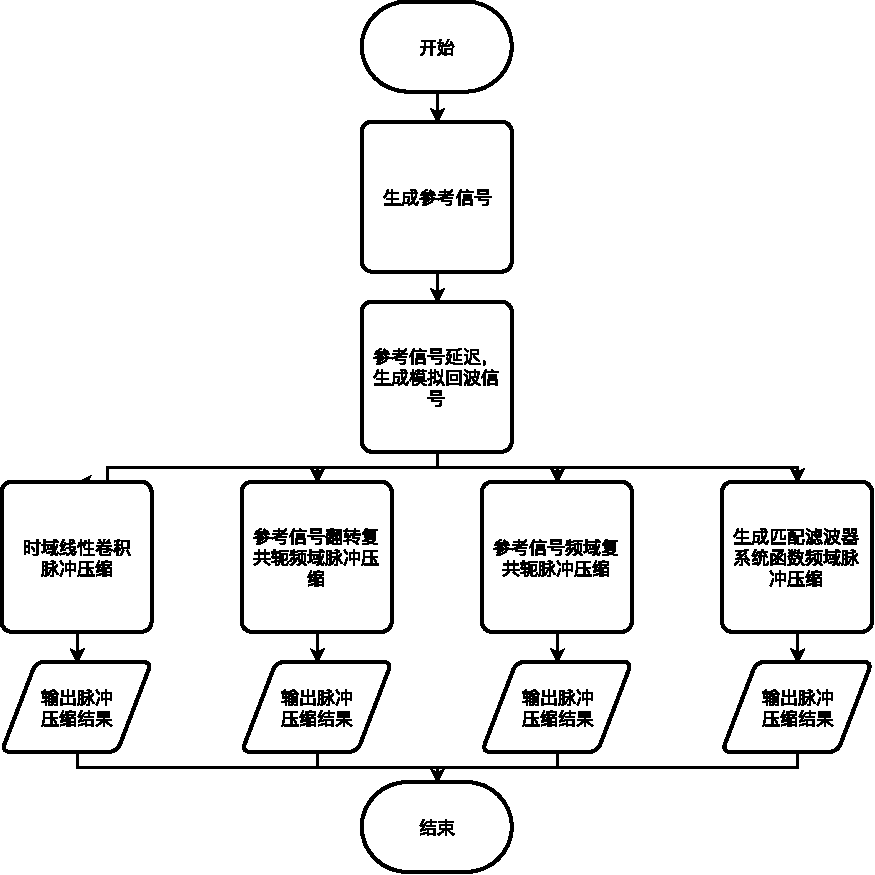
\includegraphics[width=0.6\linewidth]{figure/PulseCompression1Flowchart.pdf}
	\caption{脉冲压缩流程图}
\end{figure}
\subsection{实验程序}
\lstinputlisting[caption={脉冲压缩程序}]{"../Executable Script/Exp 11/PulseCompression.m"}
\subsection{实验结果和分析}
生成100MHz带宽的线性调频信号,对其进行频谱分析,可以得到如下图所示的频谱图。
\begin{figure}[H]
	\centering
	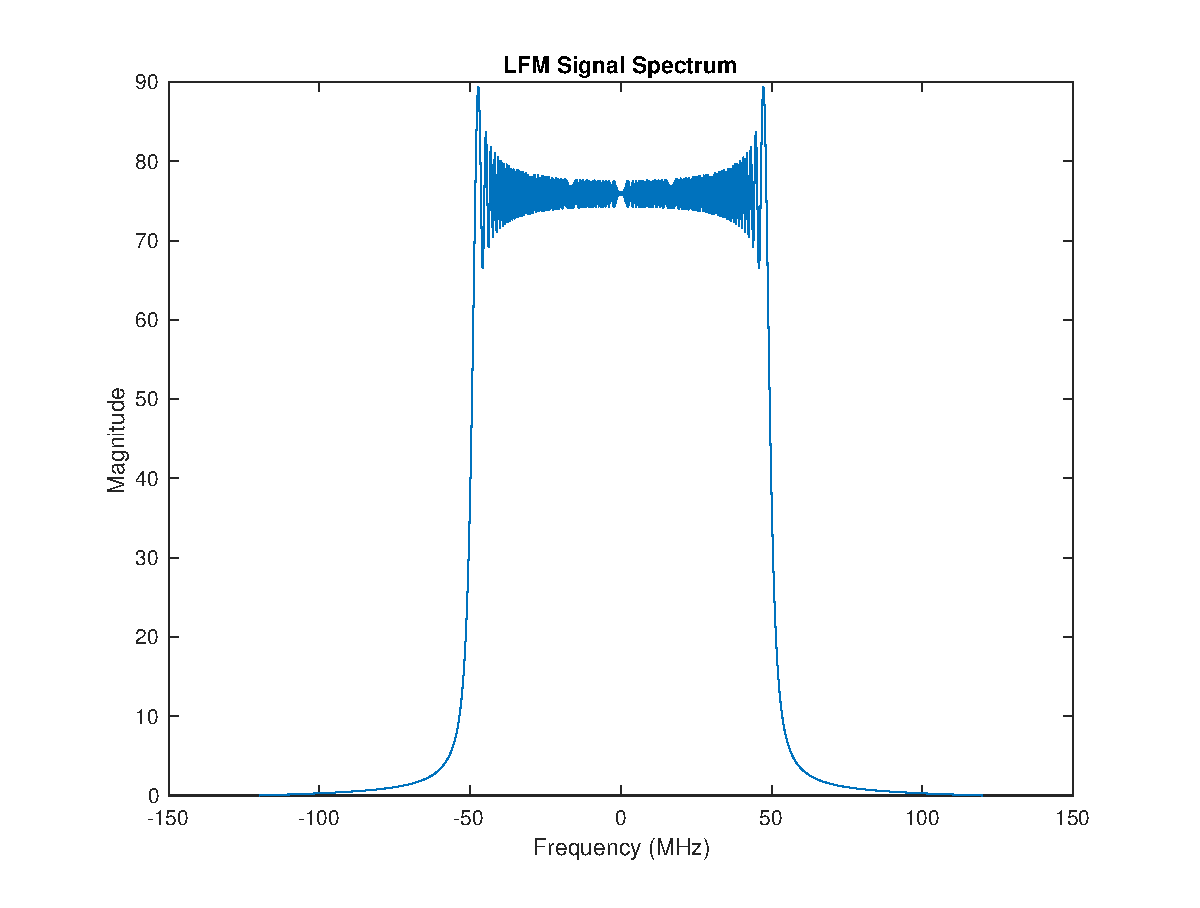
\includegraphics[width=0.7\linewidth]{figure/LFMSignalSpectrum.eps}
	\caption{线性调频信号频谱}
\end{figure}
对线性调频信号参考信号延迟17$\mu$s,生成模拟回波信号
\begin{figure}[H]
	\centering
	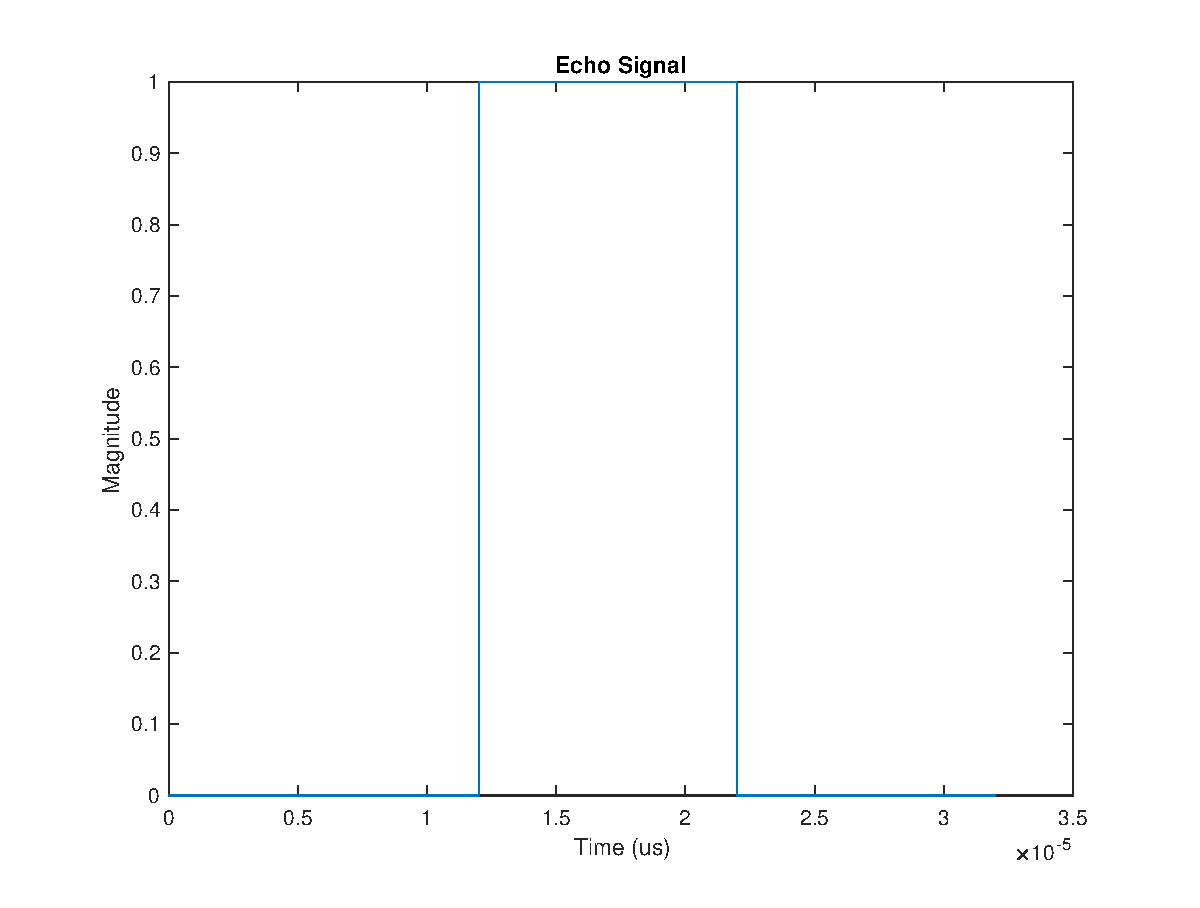
\includegraphics[width=0.7\linewidth]{figure/LFMEchoSignal.eps}
	\caption{模拟回波信号}
\end{figure}
对回波信号分别进行通过不同方式生成匹配滤波器的脉冲压缩。通过时域线性卷积可以得到脉冲压缩的结果如下图所示。
\begin{figure}[H]
	\centering
	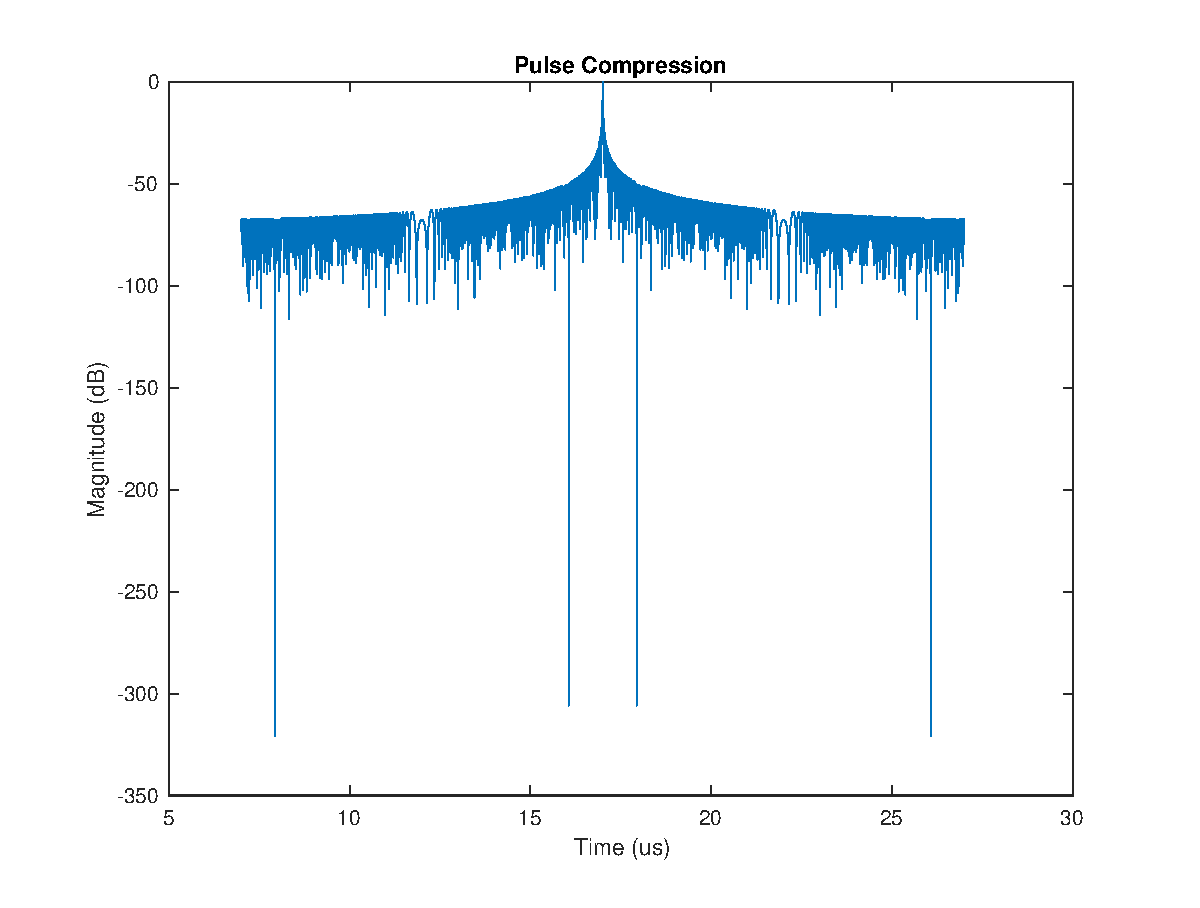
\includegraphics[width=0.7\linewidth]{figure/LinearConvolutionPulseCompression.eps}
	\caption{通过时域线性卷积实现的脉冲压缩}
\end{figure}
通过对参考信号傅立叶变换后共轭得到对匹配滤波器的频域脉冲压缩结果如下图所示。
\begin{figure}[H]
	\centering
	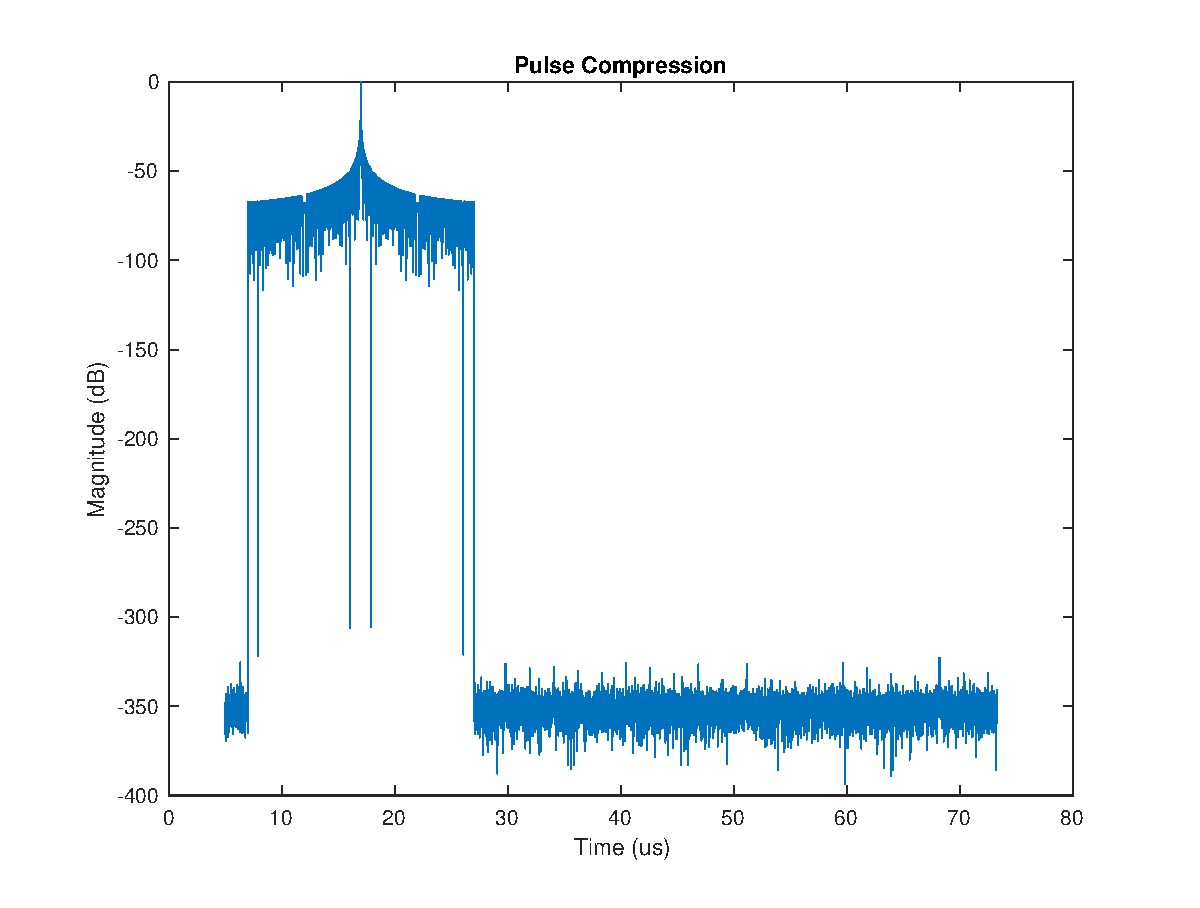
\includegraphics[width=0.7\linewidth]{figure/FFTConjuagePulseCompression.eps}
	\caption{参考信号傅立叶变换后共轭得到的匹配滤波器脉冲压缩}
\end{figure}
通过对参考信号翻转共轭傅立叶变换后得到对匹配滤波器的脉冲压缩结果如下图所示。
\begin{figure}[H]
	\centering
	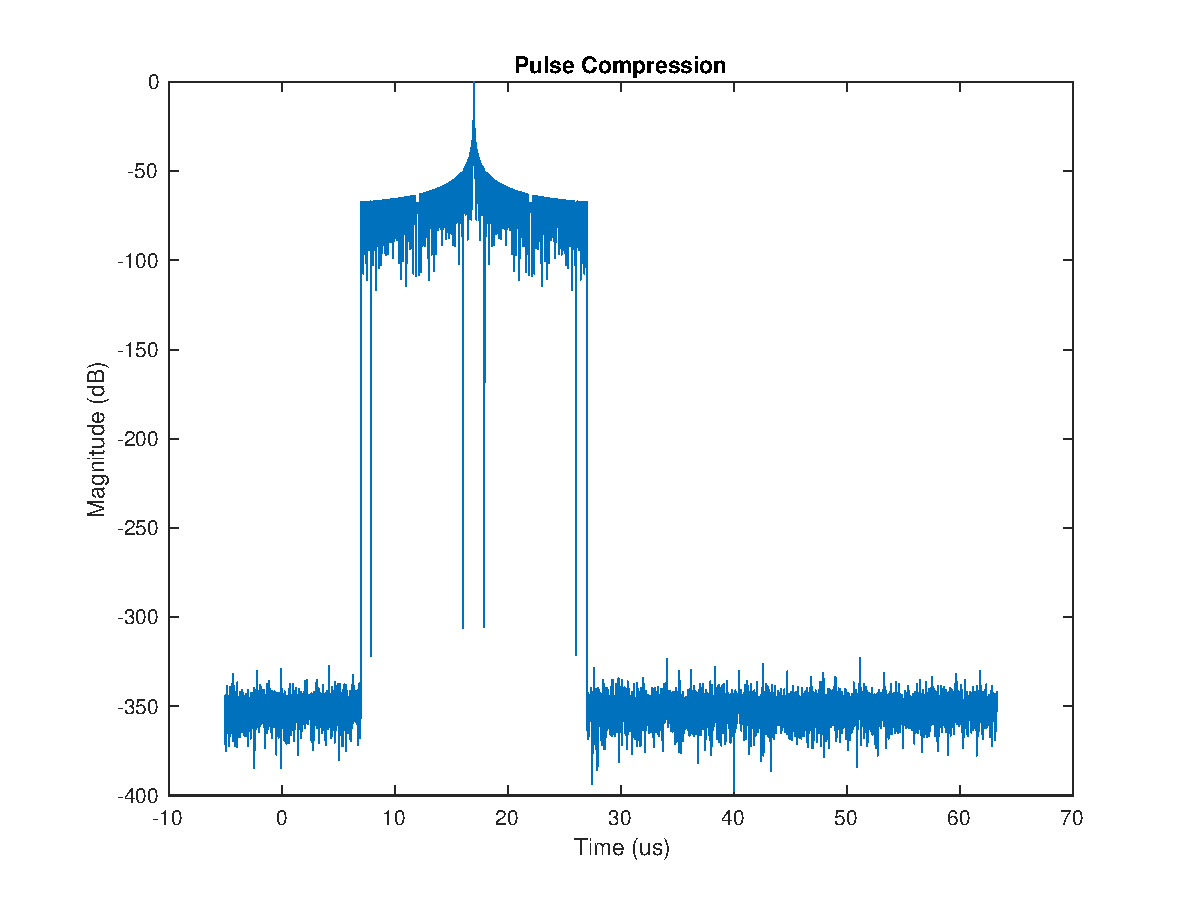
\includegraphics[width=0.7\linewidth]{figure/FilpConjugateFFTPulseCompression.eps}
	\caption{参考信号翻转共轭傅立叶变换得到的匹配滤波器脉冲压缩}
\end{figure}
可以看到,使用四种方法都可以得到脉冲压缩的结果。由于参考信号是一个关于0的共轭反对称信号,所以在进行脉冲压缩后,$\sinc$函数峰值所在的位置不尽相同,这是由于离散傅立叶变换的性质决定的,所以根据傅立叶变换的性质对脉冲压缩对结果进行相应的横坐标的设定,就可以得到正确的结果。
	\section{实验十二~线性调频信号的脉冲压缩}
	\subsection{实验目的}
进一步学习雷达信号处理中的线性调频信号及其脉冲压缩技术,分析非基带信号的脉冲压缩结果,窗效应,以及基带信号中的失配影响。
\subsection{实验原理}
\subsubsection{非基带信号的脉冲压缩}
\paragraph{非基带信号}
在时域中,非基带信号可以视为零频率时刻偏离脉冲中心的信号。设$t_c$是脉冲中心相对于$t=0$的时间偏移,则发射信号为
\begin{equation}
s(t) = \rectf{\frac{t}{T}}\exp(\jj\pi\gamma(t-t_c)^2)
\end{equation}
回波信号
\begin{equation}
s_r(t)=\rectf{\frac{t-t_0}{T}}\exp(\jj\pi\gamma(t-t_0-tc)^2)
\end{equation}
滤波器冲击相应函数
\begin{equation}
h(t)=s^*(-t)=\rectf{\frac{t}{T}}\exp\left(-\jj\pi\gamma(t+t_c)^2\right)
\end{equation}
匹配滤波器输出
\begin{equation}
s_{out}(t)=T\exp(-\jj2\pi\gamma t_c(t-t_0))\sinc(\gamma T(t-t_0))
\end{equation}
\subsubsection{点目标的质量参数}
点目标在处理后的SAR图像中表现为sinc型函数。点目标测量给出的重要的质量参数包括:
\begin{description}
	\item[冲击相应宽度(IRW)] 冲击响应的3dB主瓣宽度。冲击响应是输入为冲击函数时的系统输出。在SAR系统中,它是通过测量地面的一个单一鼓励散射体的系统响应得到的。
	\item[峰值旁瓣比(PSLR)] 最大旁瓣与主瓣的高度比,以分贝表示。sinc函数的PSLR为-13dB。SAR系统中的PSLR必须小于该值,以是的弱目标不会被邻近的强目标掩盖。PSLR一般取在-20dB左右。可以通过使用窗函数达到这一要求。
	\item[一维积分旁瓣比(ISLR)] 对冲击响应功率(幅度平方)进行积分得到。令$P_{main}$为主瓣功率,$P_{total}$为总功率,则一维$ISLR$为
	\[ ISLR=10\log_{10}\left( \frac{P_{total}-P_{main}}{P_{main}} \right) \]
	其中分子是旁瓣的总能量。主瓣宽度以峰值为中心,大小取为IRW的2-2.5被。也可以将相邻零点作为主瓣宽度,此时典型一维ISLR为-17dB。
\end{description}
\subsubsection{窗效应}
频谱近似为矩形时的PSLR为-13dB。一般认为这一PSLR过高,会淹没附近的弱目标。降低PSLR的一种方法是对频域匹配滤波器引入平滑窗,以减少主瓣到旁瓣的能量泄漏。

窗是一个对信号频谱进行加权的对称实函数。权值在信号频谱中心处最大,向频谱两边逐渐衰落。

窗能够平滑频谱,即弱化频谱边缘处的不连续性。这样会降低压缩脉冲中主瓣能量泄漏,但是会损失分辨率。因为窗是的压缩中的有效信号带宽变窄。
\paragraph{Kaiser窗}
有一个可调参数$\beta$,可以在不同应用中兼顾分辨率和旁瓣。

在时域中,长度为$T$的Kasier窗可以表示为
\begin{equation}
w_k(t, T) = \frac{I_0(\beta\sqrt{1-(2t/T)^2})}{I_0(\beta)},\quad -\frac{T}{2}\leq t\leq \frac{T}{2}
\end{equation}
其中$I_0$为零阶贝塞尔函数,$\beta$为可调整的衰减系数或平滑系数。

频域中,长度为$F$的Kasier窗可以表示为
\begin{equation}
W_k(f, F) = \frac{I_0(\beta\sqrt{1 - (2f/F)^2})}{I_0(\beta)}, \quad -\frac{F}{2}\leq f\leq\frac{F}{2}
\end{equation}
加权后的频域匹配滤波器
\begin{eqnarray}
H(f) = W_k(f, \abs{\gamma}T)\exp\left(\jj\pi\frac{f^2}{\gamma}\right)
\end{eqnarray}
加权后的时域匹配滤波器
\begin{equation}
h(t) = w_k(t, T)\exp(-\jj\pi\gamma t^2)
\end{equation}
输出信号
\begin{eqnarray}
S_{out}(f) &=& S_r(f)H(f) = W_k(f, \abs{K}T)\exp(-\jj2\pi ft_0) \\
s_{out}(t) &=& p(t - t_0)
\end{eqnarray}
\paragraph{展宽}
定义为加窗前后3dB宽度的比值。

分析不同$\beta$值时的Kaiser窗的PSLR以及相对于矩形窗的IRW展宽。$\beta$的一个典型值是2.5,与矩形窗相比,PSLR降至-21dB,分辨率扩展了1.18倍。
\subsubsection{基带信号中的失配影响}
一般用三个参数对线性调频信号的匹配滤波器加权加以描述,即持续时间、中心频率和调频率。其中,调频率的误差影响最严重。

通过对$H(f)$引入调频率wuia$\Delta K$,运用实验分析其影响。分析IRW,PSLR以及随二次相位误差QPE的变化。
\paragraph{QPE的定义}
当存在$\Delta K$时,信号与滤波器之间存在一个相位误差。设匹配滤波器的带宽与信号相同。忽略可能存在的常数相位偏移,假设匹配滤波器的中间相位与信号中间的相位匹配,则QPE为信号任意一端处的相对相位失配,此处失配最大。在此定义下,线性调频信号的QPE为
\[ QPE=\pi\Delta\gamma\left(\frac{T}{2}\right)^2 \]
\subsection{实验流程}
\begin{figure}[H]
	\centering
	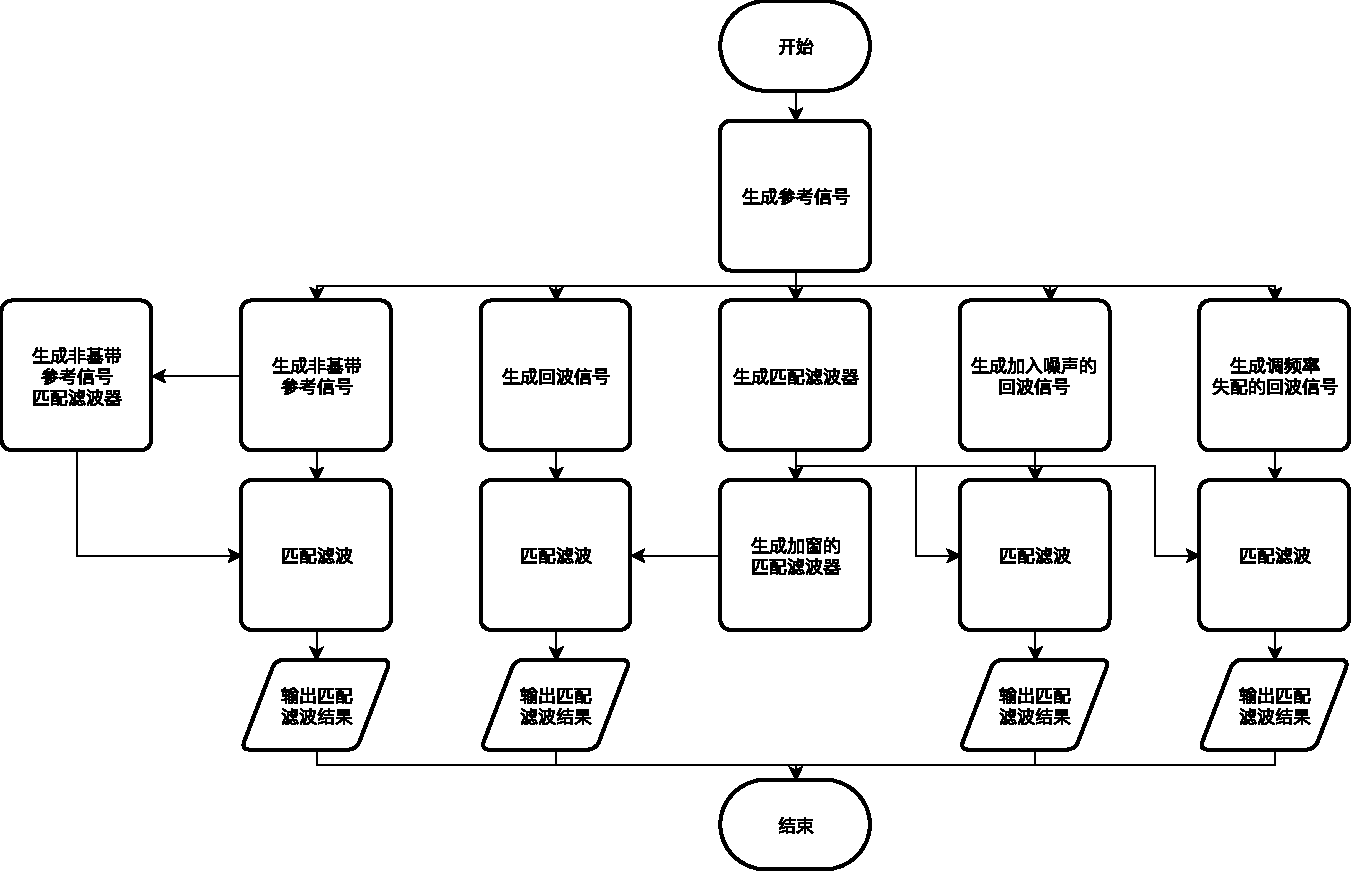
\includegraphics[width=\linewidth]{figure/AdvancedPulseCompressionFlowchart.pdf}
	\caption{脉冲压缩流程图}
\end{figure}
\subsection{实验程序}
\lstinputlisting[caption={非基带信号脉冲压缩}]{"../Executable Script/Exp 12/NoneBasebandPulseCompression.m"}
\lstinputlisting[caption={有噪声的脉冲压缩}]{"../Executable Script/Exp 12/NoisyPulseCompression.m"}
\lstinputlisting[caption={加窗的脉冲压缩}]{"../Executable Script/Exp 12/WindowedPulseCompression.m"}
\lstinputlisting[caption={调频率失配的脉冲压缩}]{"../Executable Script/Exp 12/MissingGammaPulseCompression.m"}
\subsection{实验结果和分析}
设定发射信号是100MHz带宽, 10$\mu$时宽的线性调频信号,回波信号在17$\mu$s后返回。对回波信号进行不同的处理,得到不同的结果。
\subsubsection{非基带信号的脉冲压缩}
\begin{figure}[H]
	\centering
	\begin{minipage}{0.45\linewidth}
		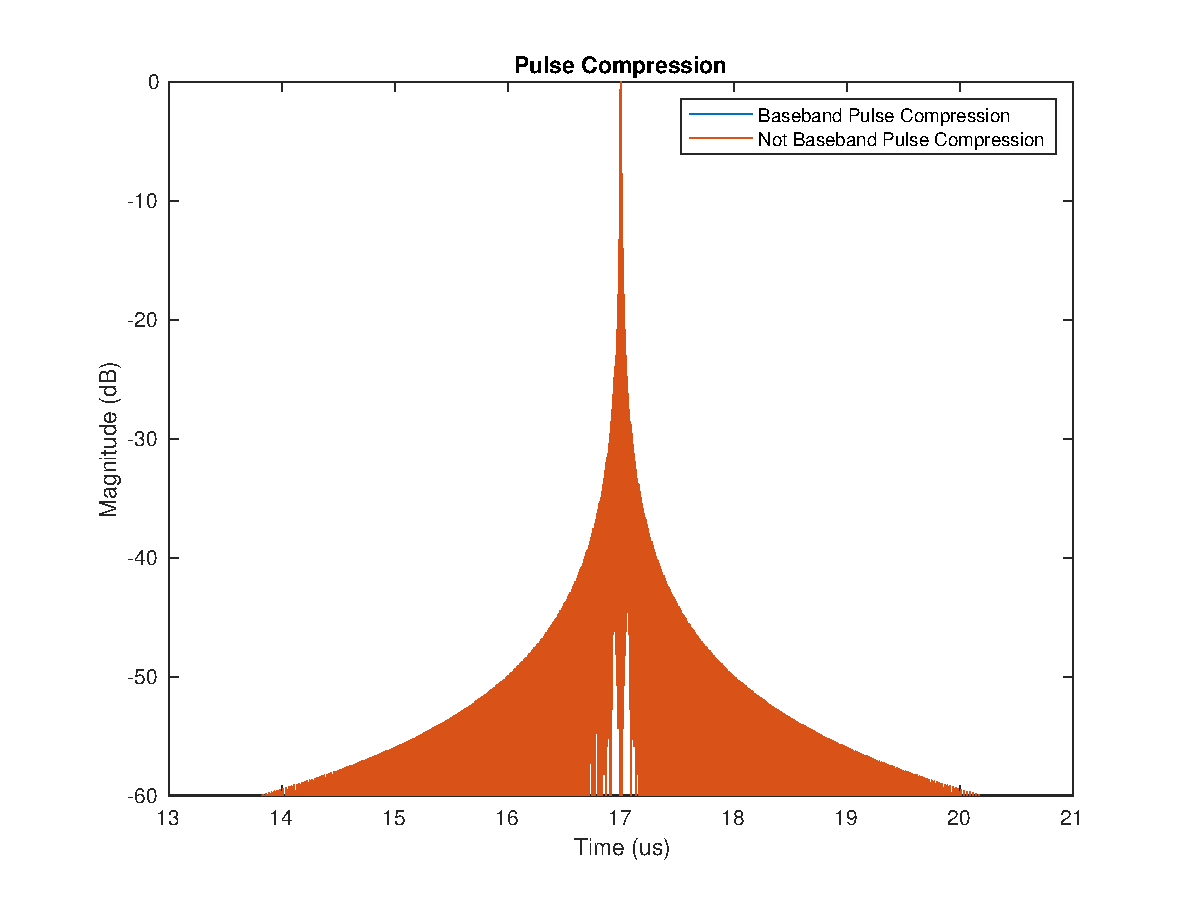
\includegraphics[width=\linewidth]{figure/NotBasebandPulseCompression.eps}
		\caption{非基带信号脉冲压缩结果(功率谱)}
	\end{minipage}
	\begin{minipage}{0.45\linewidth}
		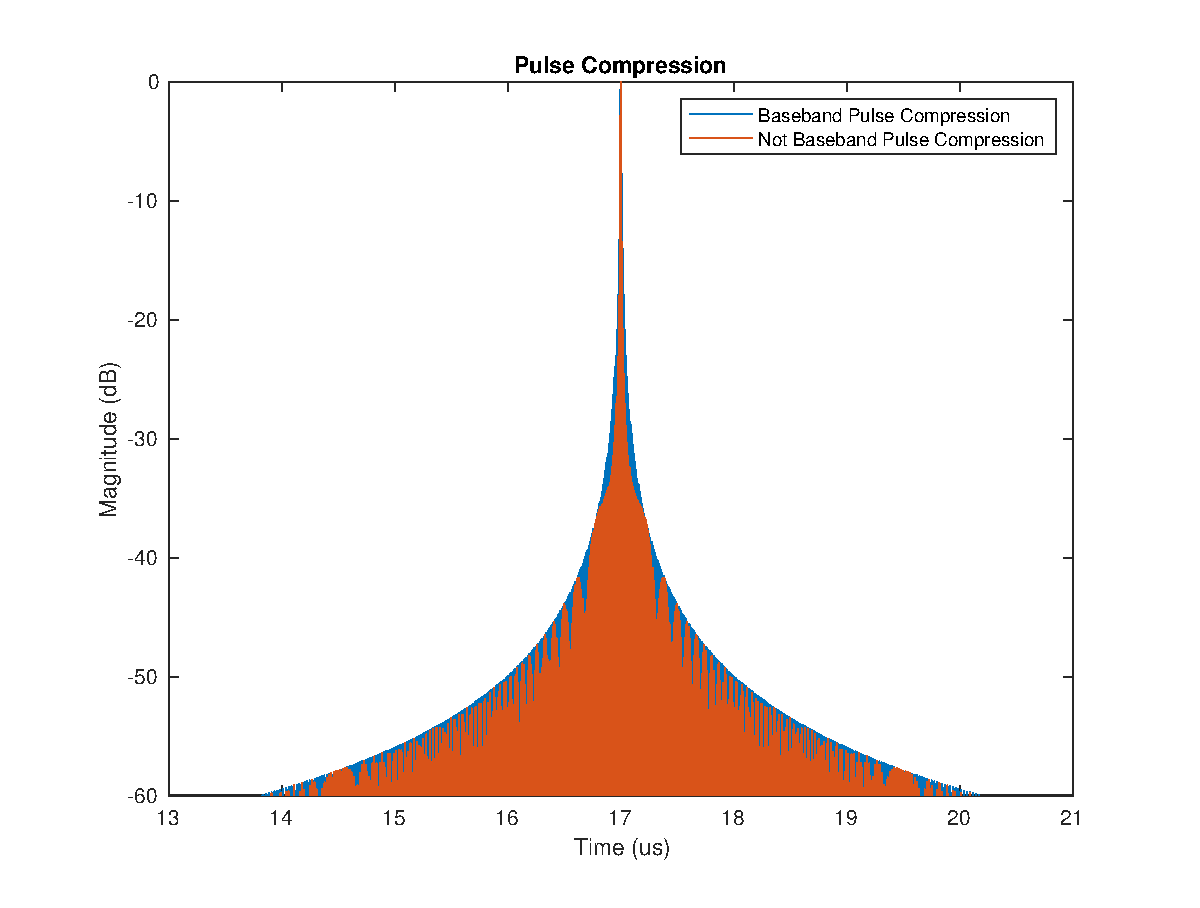
\includegraphics[width=\linewidth]{figure/NotBasebandPulseCompression_real.eps}
		\caption{非基带信号脉冲压缩结果(实部)}
	\end{minipage}
\end{figure}
可以看到非基带脉冲压缩的结果和理论计算结果相同,在功率谱上两者并没有差异。但由于零频率偏移信号中心,所以导致脉冲压缩的结果多了一个相位项,这个相位项就导致了脉冲压缩的结果乘以了一个旋转相位,这一点在脉冲压缩结果的实部上可以明显观察到,非基带信号的脉冲压缩结果的实部乘以了一个频率在信号两侧高、信号中心低的余弦信号。
\subsubsection{加入噪声的脉冲压缩}
在回波信号中加入高斯白噪声,使得回波信号信噪比达到-10dB,进行脉冲压缩,就可以得到如下图所示的脉冲压缩结果。
\singleimage{figure/NoisyPulseCompression.eps}{加入噪声的脉冲压缩}
如上图所示的结果中,可以看到噪声对信号的旁瓣造成了较大影响,使得在信号旁瓣部分能量提高了许多,但对主瓣几乎没有影响。
\subsubsection{加窗后对脉冲压缩}
对匹配滤波器的冲击响应函数加入$\beta=2.5$的Kasier窗进行脉冲压缩,可以得到如下图所示的脉冲压缩结果。
\doubleimages{figure/windowedPulseCompression.eps}{加窗后的脉冲压缩}{figure/windowedPulseCompression_zoomIn.eps}{加窗后的脉冲压缩(放大)}
可以看到加窗后的脉冲压缩的结果的旁瓣能量下降了。将图像放大后进行观察,可以看到副瓣的能量下降了7.68dB,达到了-20.96dB,3dB带宽从原来的$8.8\times 10^{-3}\mu s$展宽至$10.4\times 10^{-3}\mu s$,展宽系数1.18。
\subsubsection{调频率失配的脉冲压缩}
对模拟回波信号的调频率增加$2\%$的差异,进行脉冲压缩可以得到如下图所示的结果。
\singleimage{figure/MissmatchedGammaPulseCompression.eps}{调频率失配的脉冲压缩}
从图中可以看到,调频率的失配对脉冲压缩的结果影响非常大,它引发了主瓣的严重展宽,主瓣能量下降,这不仅对脉冲雷达的测距精度具有非常大的影响,同时对雷达的抗干扰性能、测距范围都具有很严重的不良影响。
	\section{实验十四~综合实验设计}
	\subsection{实验目的}
对于给定的遥感任务,根据本专业的专业基础课以及专业课知识,借鉴本课程前期所进行的一些实验中的原理、流程以及实验方法,自主设计给定任务的解决方案与实验方法及流程,完成实验结果的分析。
\subsection{实验原理}
\subsubsection{新型差异图像的构造方法}
在SAR图像差异图的构造中,差值法和比值法 是最常用的两种方法。图像差值法是通过对两幅同 一地区不同时刻的 SAR 图像直接逐像素相减,从而得到差异影像图。设X1与X2分别表示为同一地区 在不同时刻获取的两幅SAR图像,图像大小为
$H\times W$,则图像差值法的计算方法如下式所示:
\begin{equation}
X_d(i, j) = \abs{X_1(i, j) - X_2(i, j)}
\end{equation}
将图像的对数比法和均值比法如下式所示
\begin{eqnarray}
Xd_2(i, j) = X_1(i, j)/X_2(i, j) \\
Xd_3(i, j) = 255\times\abs{\ln(X_1(i, j)/X_2(i, j))} \\
Xd_4(i, j) = 255\times\left( 1-\min\left(\frac{\mu_1(i, j)}{\mu_2(i, j)}, \frac{\mu_2(i, j)}{\mu_1(i, j)}\right) \right)
\end{eqnarray}
所以新的差异图像构造方法为
\begin{equation}
Xd(i, j) = \frac{255\times(\ln(\mu_a(i, j) + 1) - \ln(\mu_b(i, j) + 1))}{\max(Xd) - \min(Xd)}
\end{equation}
其中,$\mu_a$表示的是两幅图像中灰度值总和较大的图像中以坐标(i,j)为中心的3x3邻域 窗口内像素的灰度均值,$\mu_b$表示的是两幅图像中灰度值总和较小的图像中以坐标(i,j)为中心的3x3邻域 窗口内像素的灰度均值。
\subsection{实验流程}
\begin{figure}[H]
	\centering
	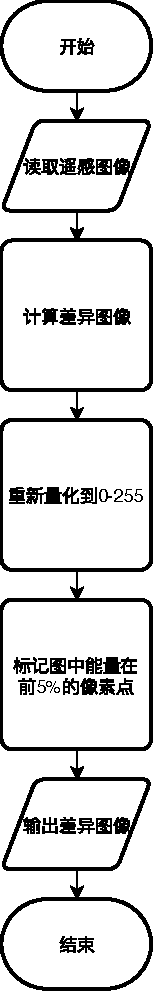
\includegraphics[width=0.15\linewidth]{figure/FinalFlowchart.pdf}
	\caption{实验过程流程图}
\end{figure}
\subsection{实验程序}
\lstinputlisting[caption={图像差异检测程序}]{"../Executable Script/Exp 14/main.m"}
\lstinputlisting[caption={新型差异图像检测函数FusionDifferDetection}]{"../Function Library/FusionDifferDetection.m"}
\lstinputlisting[caption={自动重新量化灰度值函数AutoGrayScale}]{"../Function Library/AutoGrayScale.m"}
\lstinputlisting[caption={自动二值化图像函数AutoBinarizeImage}]{"../Function Library/AutoBinarizeImage.m"}
\lstinputlisting[caption={虚警率计算函数ClassificationFalseAlarmRate}]{"../Function Library/ClassificationFalseAlarmRate.m"}
\lstinputlisting[caption={漏警率计算函数ClassificationMissingAlarmRate}]{"../Function Library/ClassificationMissingAlarmRate.m"}
\subsection{实验结果和分析}
对如下图所示的遥感图像进行差异检测
\doubleimages{figure/san_1.bmp}{遥感图像1}{figure/san_2.bmp}{遥感图像2}
可以得到如下图所示的结果
\singleimage{figure/FinalResult}{差异检测结果}
经过计算得到虚警率$6.46\%$,漏警率$20.02\%$。
\end{document}